\subsection{Гипербола}
 
\textsl{Гипербола} --- геометрическое место точек M Евклидовой плоскости, для которых абсолютное значение разности расстояний от $M$ до двух выделенных точек $F_1$ и $F_2$ (называемых фокусами) постоянно и равно удвоенной действительной полуоси гиперболы.
\begin{equation}
\bigl||F_1M|-|F_2M|\bigr|=2a
\end{equation}
\textbf{Основные формулы для гиперболы:}
\begin{equation}
c^2=a^2+b^2
\end{equation}
Эксцентриситет гиперболы $e>1$ и вычисляется по формуле:
\begin{equation}
e=\frac{c}{a}
\end{equation}
Перецентрическое расстояние гиперболы вычисляется по следующей формуле:
\begin{equation}
q=a(e-1)
\end{equation}
Фокальный параметр вычисляется также, как и для эллипса:
\begin{equation}
p=\frac{b^2}{a}
\end{equation}
\textbf{Уравнение гиперболы:}

Канонический вид:
\begin{equation}
\frac{x^2}{a^2}-\frac{y^2}{b^2}=1
\end{equation}

Если полюс находится в фокусе гиперболы, а вершина гиперболы лежит на продолжении полярной оси, то, уравнение гиперболы в полярных координатах имеет следующий вид:
\begin{equation}
r=\frac{p}{1-e\cos\phi}
\end{equation}

Уравнение двух асимптот имеет следующий вид:
\begin{equation}
\frac{x}{a}\pm\frac{y}{b}=0
\end{equation}

Эксцентриситет, действительная и мнимая полуоси соотносятся следующим образом:
\begin{equation}
b^2=a^2(e^2-1)
\end{equation}
\textbf{Оптическое свойство гиперболы:}

Свет от источника, находящегося в одном из фокусов гиперболы, отражается второй ветвью гиперболы таким образом, что продолжения отраженных лучей пересекаются во втором фокусе.
\begin{figure}[h!]
\centering
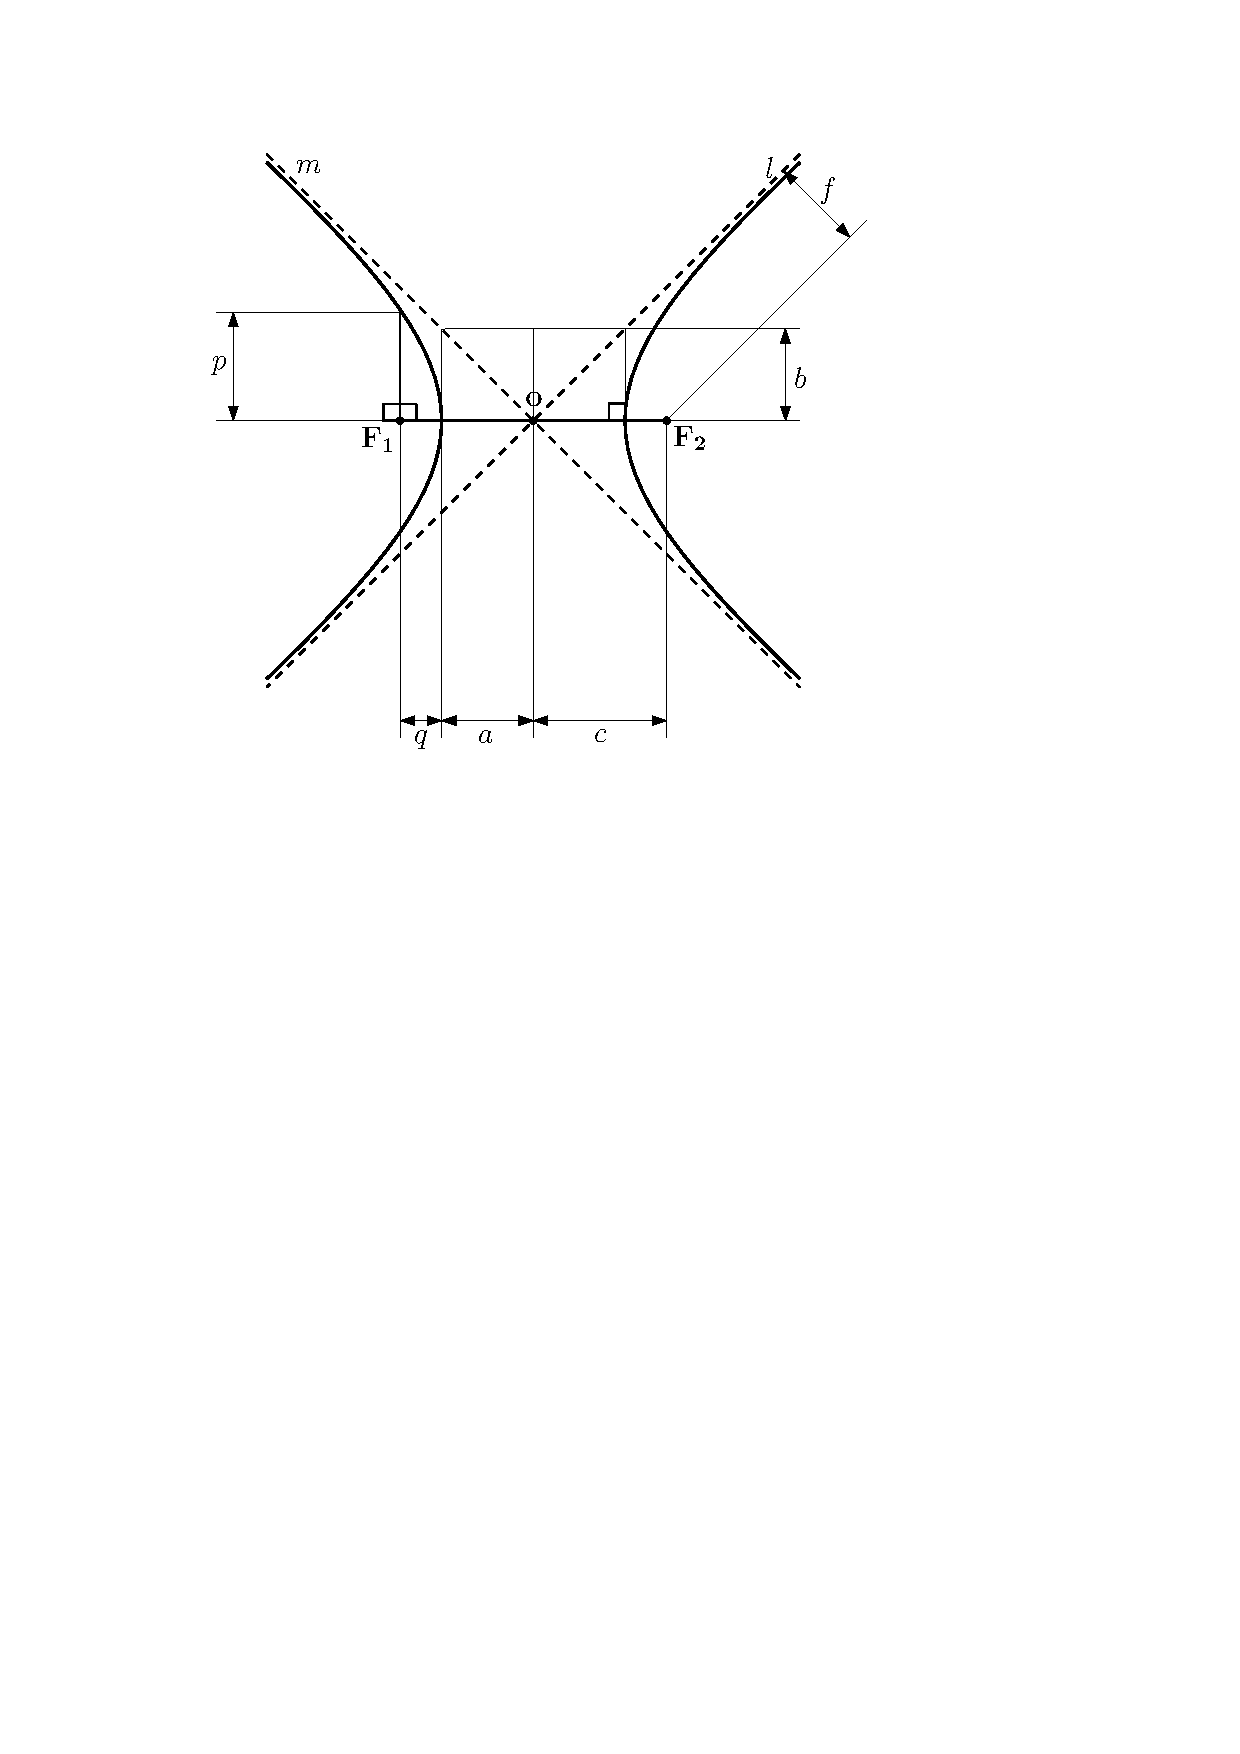
\includegraphics[width = 0.6\textwidth]{Hiperbola}
\caption{Гипербола \label{pic:the-pic}}
\end{figure}